\documentclass[tikz,border=10pt]{standalone}
\usepackage{amssymb}
\usetikzlibrary{arrows.meta, bending, decorations.markings, calc, shapes.geometric}

% Definição de estilos
\tikzset{
  glueArrow/.style={-{Stealth[length=3mm]}, very thick, shorten >=2pt, shorten <=2pt},
  pathArrow/.style args={#1}{
    postaction={decorate},
    decoration={markings,
      mark=at position #1 with {\arrow[scale=1.5]{Stealth}}
    }
  },
  cycleLines/.style={very thick, draw=black}, % Garante que as linhas sejam pretas
  % --- ESTILOS DE COR APENAS PARA OS NÓS ---
  dotBase/.style={circle, inner sep=1.2pt},
  % Azul para a direção horizontal (x^n-1)
  dotBlue/.style={dotBase, fill=blue!70!cyan},
  dotBlueBack/.style={dotBase, fill=blue!30!gray}, 
  % Vermelho para a direção vertical (Z_p)
  dotRed/.style={dotBase, fill=red!70!orange},
  dotRedBack/.style={dotBase, fill=red!30!gray} 
}

\begin{document}

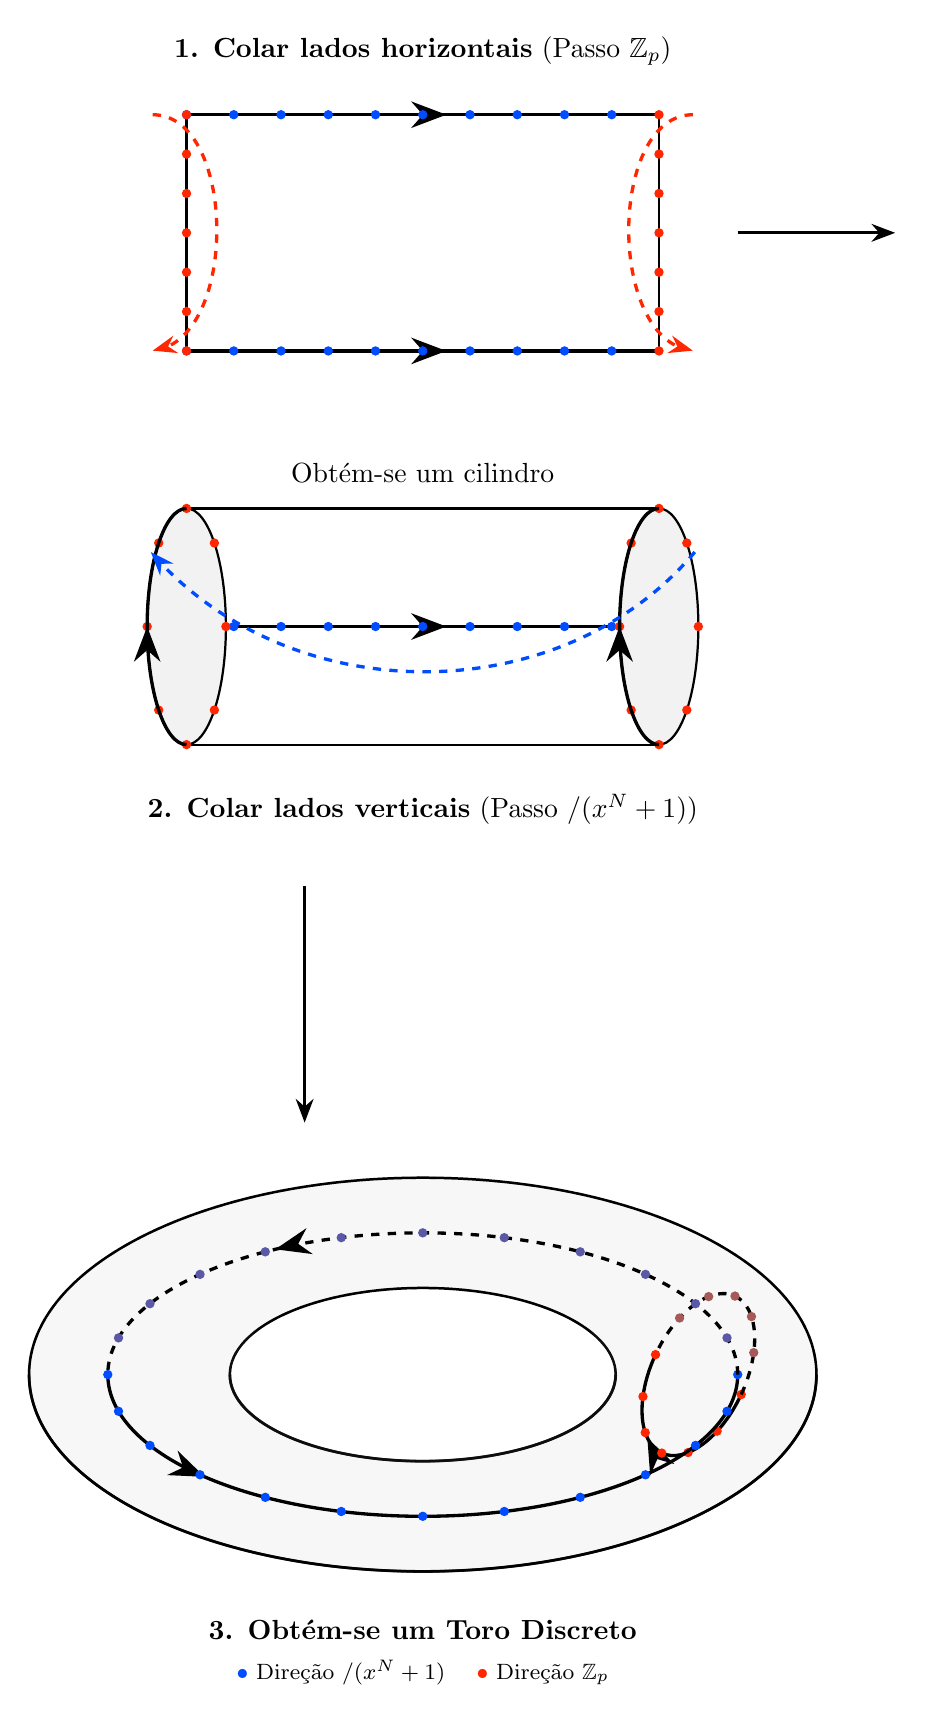
\begin{tikzpicture}
  %% --- PARTE 1: O RETÂNGULO ---
  \begin{scope}[yshift=0cm]
    % Coordenadas
    \coordinate (A) at (0, 0);
    \coordinate (B) at (6, 0);
    \coordinate (C) at (6, 3);
    \coordinate (D) at (0, 3);

    % Desenho do contorno (PRETO)
    \draw[thick] (A) -- (B) -- (C) -- (D) -- cycle;

    % Linhas de direção (PRETAS)
    \draw[cycleLines, pathArrow=0.55] (A) -- (B);
    \draw[cycleLines, pathArrow=0.55] (D) -- (C);

    % --- PONTOS DISCRETOS COLORIDOS ---
    % Pontos horizontais (Azul - grau n)
    \foreach \x in {0, 0.6, ..., 6} {
        \node[dotBlue] at (\x, 0) {};
        \node[dotBlue] at (\x, 3) {};
    }
    % Pontos verticais (Vermelho - Z_p)
    \foreach \y in {0, 0.5, ..., 3} {
        \node[dotRed] at (0, \y) {};
        \node[dotRed] at (6, \y) {};
    }

    % Setas de colagem (Mantive coloridas apenas para indicar QUEM está sendo colado com quem, 
    % mas se preferir preto, basta remover a cor)
    \draw[glueArrow, dashed, bend left=90, red!70!orange]  ($(D)+(-0.5,0)$) to ($(A)+(-0.5,0)$);
    \draw[glueArrow, dashed, bend right=90, red!70!orange] ($(C)+(0.5,0)$)  to ($(B)+(0.5,0)$);

    \node[above] at (3, 3.5) {\textbf{1. Colar lados horizontais} (Passo $\mathbb{Z}_p$)};
    
    % Transição
    \draw[-{Stealth[length=3mm]}, very thick] (7, 1.5) -- (9, 1.5);
  \end{scope}


  %% --- PARTE 2: O CILINDRO ---
  \begin{scope}[yshift=-5cm]
    % Corpo
    \draw[thick] (0, 3) -- (6, 3);
    \draw[thick] (0, 0) -- (6, 0);

    % Costura horizontal (LINHA PRETA)
    \draw[cycleLines, pathArrow=0.55] (0, 1.5) -- (6, 1.5);
    % Pontos na costura (AZUIS)
    \foreach \x in {0, 0.6, ..., 6} {
        \node[dotBlue] at (\x, 1.5) {};
    }

    % Tampas
    \draw[thick, fill=gray!10] (0, 1.5) ellipse (0.5 and 1.5);
    % Pontos na tampa esquerda (VERMELHOS)
    \foreach \ang in {0, 45, ..., 315} {
        \node[dotRed] at ({0 + 0.5*cos(\ang)}, {1.5 + 1.5*sin(\ang)}) {};
    }
    
    \draw[thick, fill=gray!10] (6, 1.5) ellipse (0.5 and 1.5);
    % Pontos na tampa direita (VERMELHOS)
    \foreach \ang in {0, 45, ..., 315} {
        \node[dotRed] at ({6 + 0.5*cos(\ang)}, {1.5 + 1.5*sin(\ang)}) {};
    }

    % Ciclos verticais nas tampas (LINHAS PRETAS)
    \draw[cycleLines, pathArrow=0.5] (0,0) arc (270:90:0.5 and 1.5);
    \draw[cycleLines, pathArrow=0.5] (6,0) arc (270:90:0.5 and 1.5);

    % Seta de colagem (Azul para indicar direção horizontal sendo unida)
    \draw[glueArrow, dashed, bend left=50, blue!70!cyan] (6.5, 2.5) to (-0.5, 2.5);

    \node[above] at (3, 3.2) {Obtém-se um cilindro};
    \node[below] at (3, -0.5) {\textbf{2. Colar lados verticais} (Passo $/(x^N  +1)$)};
  \end{scope}

  % Transição
  \draw[-{Stealth[length=3mm]}, very thick] (1.5, -6.8) -- (1.5, -9.8);


  %% --- PARTE 3: O TORO ---
  \begin{scope}[yshift=-13cm, xshift=3cm]
    % Contorno e Buraco
   % --- TORO (2D) mais "donut" + transparente (robusto) ---
\def\RoutX{5}
\def\RoutY{2.5}
\def\RinX{2.45}
\def\RinY{1.10}

% Corpo como anel transparente (buraco real)
\path[even odd rule,
      fill=gray!50, fill opacity=0.13,
      draw=black, line width=0.9pt]
  (0,0) ellipse[x radius=\RoutX cm, y radius=\RoutY cm]
  (0,0) ellipse[x radius=\RinX cm,  y radius=\RinY cm];

% RIM externo: trás (tracejado) / frente (contínuo)
\draw[black, opacity=0.30, dashed, line width=0.9pt]
  (-\RoutX,0) arc[start angle=180, end angle=0,
                  x radius=\RoutX cm, y radius=\RoutY cm];
\draw[black, opacity=0.85, line width=1.0pt]
  (\RoutX,0) arc[start angle=0, end angle=-180,
                 x radius=\RoutX cm, y radius=\RoutY cm];

% RIM interno: trás (tracejado) / frente (contínuo)
\draw[black, opacity=0.30, dashed, line width=0.9pt]
  (-\RinX,0) arc[start angle=180, end angle=0,
                 x radius=\RinX cm, y radius=\RinY cm];
\draw[black, opacity=0.85, line width=1.0pt]
  (\RinX,0) arc[start angle=0, end angle=-180,
                x radius=\RinX cm, y radius=\RinY cm];

% Highlight (opcional)
\path[even odd rule, fill=white, fill opacity=0.05]
  (0,0.22) ellipse[x radius=4.6cm, y radius=2.15cm]
  (0,0.22) ellipse[x radius=2.25cm, y radius=1.02cm];
   % --- CICLO MENOR (Mod p) ---
    \coordinate (mC) at (3.5,0); 
    \begin{scope}[rotate around={-25:(mC)}]
      % Frente (Contínua) - LINHA PRETA
      \draw[cycleLines, pathArrow=0.6] ($(mC)+(0.6,0)$) arc (0:-180:0.6 and 1.1);
      
      % Pontos na frente (VERMELHOS VIVOS)
      \foreach \ang in {0, -30, ..., -180} {
         \node[dotRed] at ($(mC)+({0.6*cos(\ang)}, {1.1*sin(\ang)})$) {};
      }

      % Trás (Tracejada) - LINHA PRETA
      \draw[cycleLines, dashed] ($(mC)+(0.6,0)$) arc (0:180:0.6 and 1.1);
      
      % Pontos atrás (VERMELHOS ACINZENTADOS)
      \foreach \ang in {30, 60, ..., 150} {
         \node[dotRedBack] at ($(mC)+({0.6*cos(\ang)}, {1.1*sin(\ang)})$) {};
      }
    \end{scope}

    % --- CICLO MAIOR (Mod x^n-1) ---
    % Linha Frente (PRETA)
    \draw[cycleLines, pathArrow=0.2] (-4,0) arc (180:360:4 and 1.8);
    
    % Pontos no ciclo maior frente (AZUIS VIVOS)
    \foreach \ang in {180, 195, ..., 360} {
        \node[dotBlue] at ({4*cos(\ang)}, {1.8*sin(\ang)}) {};
    }

    % Linha Trás (PRETA TRACEJADA)
    \draw[cycleLines, dashed, pathArrow=0.7] (4,0) arc (0:180:4 and 1.8);
    
    % Pontos no ciclo maior trás (AZUIS ACINZENTADOS)
    \foreach \ang in {15, 30, ..., 165} {
        \node[dotBlueBack] at ({4*cos(\ang)}, {1.8*sin(\ang)}) {};
    }

    \node[below] at (0, -3) {\textbf{3. Obtém-se um Toro Discreto}};
    % Legenda
    \node[below, font=\footnotesize] at (0, -3.5) {\textcolor{blue!70!cyan}{$\bullet$} Direção $/(x^N+1)$ \quad \textcolor{red!70!orange}{$\bullet$} Direção $\mathbb{Z}_p$};
  \end{scope}

\end{tikzpicture}
\end{document}